\documentclass[spec, och, labwork]{shiza}
% параметр - тип обучения - одно из значений:
%    spec     - специальность
%    bachelor - бакалавриат (по умолчанию)
%    master   - магистратура
% параметр - форма обучения - одно из значений:
%    och   - очное (по умолчанию)
%    zaoch - заочное
% параметр - тип работы - одно из значений:
%    referat    - реферат
%    coursework - курсовая работа (по умолчанию)
%    diploma    - дипломная работа
%    pract      - отчет по практике
% параметр - включение шрифта
%    times    - включение шрифта Times New Roman (если установлен)
%               по умолчанию выключен
\usepackage{subfigure}
\usepackage{tikz,pgfplots}
\pgfplotsset{compat=1.5}
\usepackage{float}

%\usepackage{titlesec}
\setcounter{secnumdepth}{4}
%\titleformat{\paragraph}
%{\normalfont\normalsize}{\theparagraph}{1em}{}
%\titlespacing*{\paragraph}
%{35.5pt}{3.25ex plus 1ex minus .2ex}{1.5ex plus .2ex}

\titleformat{\paragraph}[block]
{\hspace{1.25cm}\normalfont}
{\theparagraph}{1ex}{}
\titlespacing{\paragraph}
{0cm}{2ex plus 1ex minus .2ex}{.4ex plus.2ex}

% --------------------------------------------------------------------------%


\usepackage[T2A]{fontenc}
\usepackage[utf8]{inputenc}
\usepackage{graphicx}
\graphicspath{ {./images/} }
\usepackage{tempora}

\usepackage[sort,compress]{cite}
\usepackage{amsmath}
\usepackage{amssymb}
\usepackage{amsthm}
\usepackage{fancyvrb}
\usepackage{listings}
\usepackage{listingsutf8}
\usepackage{longtable}
\usepackage{array}
\usepackage[english,russian]{babel}

% \usepackage[colorlinks=true]{hyperref}
\usepackage{url}

\usepackage{underscore}
\usepackage{setspace}
\usepackage{indentfirst} 
\usepackage{mathtools}
\usepackage{amsfonts}
\usepackage{enumitem}
\usepackage{tikz}
\usepackage{minted}

\newcommand{\eqdef}{\stackrel {\rm def}{=}}
\newcommand{\specialcell}[2][c]{%
\begin{tabular}[#1]{@{}c@{}}#2\end{tabular}}

\renewcommand\theFancyVerbLine{\small\arabic{FancyVerbLine}}

\newtheorem{lem}{Лемма}

\begin{document}

% Кафедра (в родительном падеже)
\chair{}

% Тема работы
\title{Регистры}

% Курс
\course{3}

% Группа
\group{331}

% Факультет (в родительном падеже) (по умолчанию "факультета КНиИТ")
\department{факультета КНиИТ}

% Специальность/направление код - наименование
%\napravlenie{09.03.04 "--- Программная инженерия}
%\napravlenie{010500 "--- Математическое обеспечение и администрирование информационных систем}
%\napravlenie{230100 "--- Информатика и вычислительная техника}
%\napravlenie{231000 "--- Программная инженерия}
\napravlenie{10.05.01 "--- Компьютерная безопасность}

% Для студентки. Для работы студента следующая команда не нужна.
% \studenttitle{Студентки}

% Фамилия, имя, отчество в родительном падеже
\author{Стаина Романа Игоревича и Токарева Никиты Сергеевича}

% Заведующий кафедрой
% \chtitle{} % степень, звание
% \chname{}

%Научный руководитель (для реферата преподаватель проверяющий работу)
\satitle{аспирант} %должность, степень, звание
\saname{А. А. Мартышкин}

% Руководитель практики от организации (только для практики,
% для остальных типов работ не используется)
% \patitle{к.ф.-м.н.}
% \paname{С.~В.~Миронов}

% Семестр (только для практики, для остальных
% типов работ не используется)
%\term{8}

% Наименование практики (только для практики, для остальных
% типов работ не используется)
%\practtype{преддипломная}

% Продолжительность практики (количество недель) (только для практики,
% для остальных типов работ не используется)
%\duration{4}

% Даты начала и окончания практики (только для практики, для остальных
% типов работ не используется)
%\practStart{30.04.2019}
%\practFinish{27.05.2019}

% Год выполнения отчета
\date{2022}

\maketitle

% Включение нумерации рисунков, формул и таблиц по разделам
% (по умолчанию - нумерация сквозная)
% (допускается оба вида нумерации)
% \secNumbering

%-------------------------------------------------------------------------------------------
\section{Цель работы:}

  Ознакомление с устройством и функционированием регистров и регистровой памяти; испытание интегрального универсального регистра сдвига.

  \textbf{Задание 1.}

  Построим схему и испытаем универсальный регистр сдвига:

  \begin{figure}[H]
    \centering     
    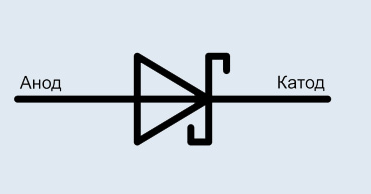
\includegraphics[width=0.7\textwidth]{photo/1}
    \caption{Реализация схемы из задания 1}
  \end{figure}

  \textbf{Задание 2.}

  Составим план исследования параллельного регистра сдвига, заполнив ячейки памяти генератора.

  \begin{figure}[H]
    \centering     
    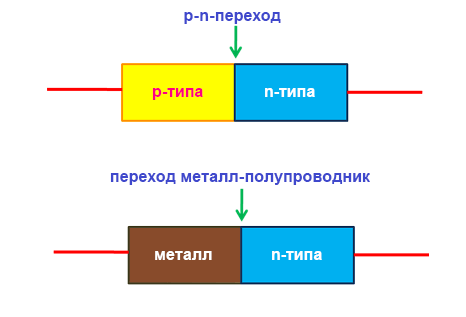
\includegraphics[width=0.7\textwidth]{photo/2}
    \caption{План исследования параллельного регистра сдвига}
  \end{figure}

  Временная диаграмма сигналов на входах и выходах регистра представлена на рисунке 3.

  \begin{figure}[H]
    \centering     
    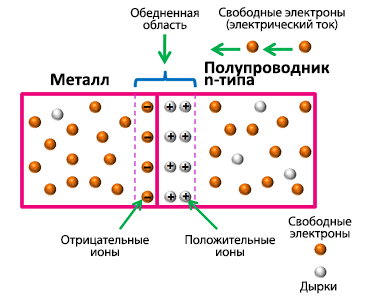
\includegraphics[width=0.7\textwidth]{photo/3}
    \caption{Временная диаграмма сигналов на входах и выходах регистра}
  \end{figure}

  \textbf{Задание 3.}

  Построим новую схему, как показано на рисунке 4.

  \begin{figure}[H]
    \centering     
    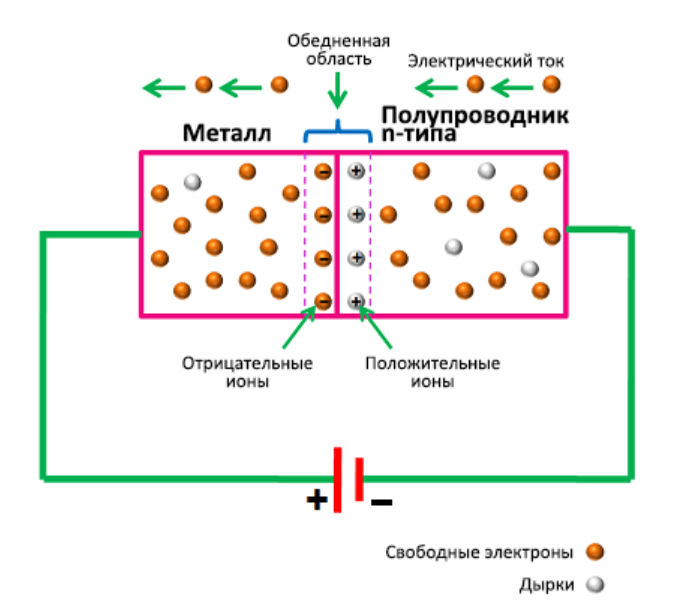
\includegraphics[width=0.7\textwidth]{photo/4}
    \caption{Построение новой схемы}
  \end{figure}

  Исследуем микросхему в качестве последовательного регистра сдвига влево. Нужно подать на управляющий вход S0 высокий уровень напряжения, а на вход $S1$ – низкий уровень, то есть установить $S0 = 1$ и $S1 = 0$, и подавать в последовательной форме на вход $SR$ данные, например 1, 0, 1 и 0, которые записываются в разряд $A$ и передаются на выход $QA$.

  \begin{figure}[H]
    \centering     
    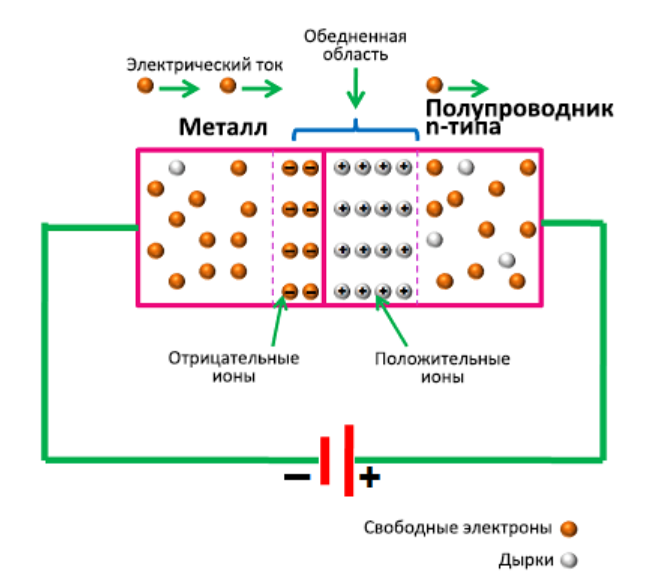
\includegraphics[width=0.7\textwidth]{photo/5}
    \caption{Анализ микросхемы}
  \end{figure}

  Регистр последовательно сдвигает влево эти сигналы от $QA$ к $QD$, на выходе $QD$ они теряются. При установке $S1 = 0$ и $S1 = 1$ и подаче на вход $SL$ данных в последовательной форме, например 1, 0, 0 и 1, которые записываются в разряд $D$ (и передаются на выход $QD$), микросхема работает в режиме последовательного регистра сдвига вправо (без кольцевого перемещения данных): сигналы 1, 0, 0 и 1 сдвигаются по направлению к разряду $A$, на выходе $QA$ они теряются.

  \textbf{Задание 4.}

  Заполним ячейки памяти генератора произвольными 4-разрядными кодовыми комбинациями, вводимыми последовательно в регистр A.

  \begin{figure}[H]
    \centering     
    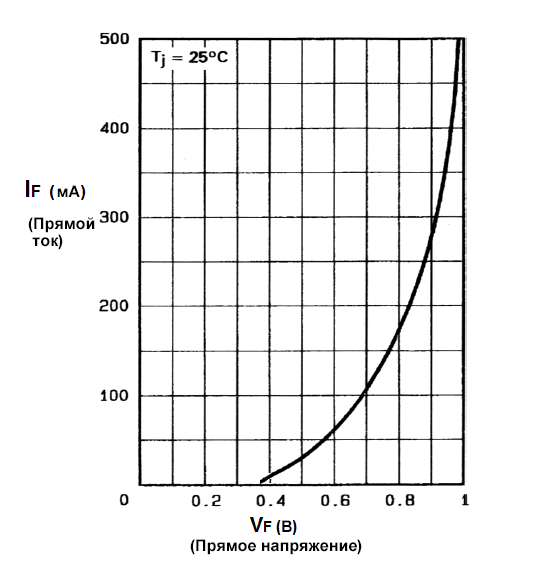
\includegraphics[width=0.7\textwidth]{photo/6}
    \caption{Анализ микросхемы после заполнения ячеек памяти генератора}
  \end{figure}

  \textbf{Вывод:} ознакомились с устройством и функционированием регистров и регистровой памяти; испытали интегральный универсальный регистр сдвига.

  \section{Тестовые задания к работе 33:}

  \begin{enumerate}
    \item Укажите функции, которые в общем случае может выполнять регистр:
    
    Ответ: 
    \begin{itemize}
      \item Обнуление (очистку) хранимой информации, запись входной информации в последовательном или в параллельном коде;
      \item Преобразование информации путем ее сдвига под воздействием тактовых импульсов;
      \item Хранение информации, ее сдвиг вправо и влево, выдачу хранимой информации в последовательном или в параллельном коде.
    \end{itemize}

    \item В параллельном регистре с приходом каждого тактового испульса информация на выходах поразрядно свигается в направлении от выхода $QD$ к выходу $QA$. Укажите, как называют такой регистр:
    
    Ответ: Регистр прямого сдвига.

    \item Укажите, какие регистры выполняют со статическим управлением:
    
    Ответ: Последовательные.

    \item Укажите, при каких уровнях сигналов на управляющих входах $S0$ и $S1$ информационные входы реверсивного регистра $74HC194\_4V$:
  
    Ответ: $S0 = 0$ и $S1 = 0$

    \item Укажите, в какой разряд вводится информация последовательного регистра $74HC194\_4V$ при $S0 = 1$, $S1 = 0$ на управляющих входах и сигналах $SR = 1$ и $CLR = 1$:
  
    Ответ: В разряд $A$.

    \item Укажите, при каикх уравнях управляющих сигналов $S0$ и $S1$ разрешена запись информации в параллельный регистр $74HC194\_4V$:
    
    Ответ: $S0 = 1$ и $S1 = 1$

    \item Укажите, разрешено ли последовательное перемещение сигналов в триггерной подсистеме параллельного регистра $74HC194\_4V$ во время записи информации:
    
    Ответ: Нет.

    \item Укажите, сколько входов имеет последовательный регистр с динамическим управлением:
    
    Ответ: Три: один информационный, вход для тактовых импульсов и установочный вход.

    \item Укажите, чем отличается динамическое управление регистрами от статического управления:
    
    Ответ: При динамическом управлении запоминание сигналов, действующих на информационных входах регистра, происходит во входных емкостях МДП-транзисторов в момент изменения значения сигнала на входе синхронизации, а в статических регистрах, построенных, например, $RS$-триггерах, сигналы действуют в момент их поступления на информационные входы.
    
  \end{enumerate}

\end{document}